% This file was created with tikzplotlib v0.10.1.
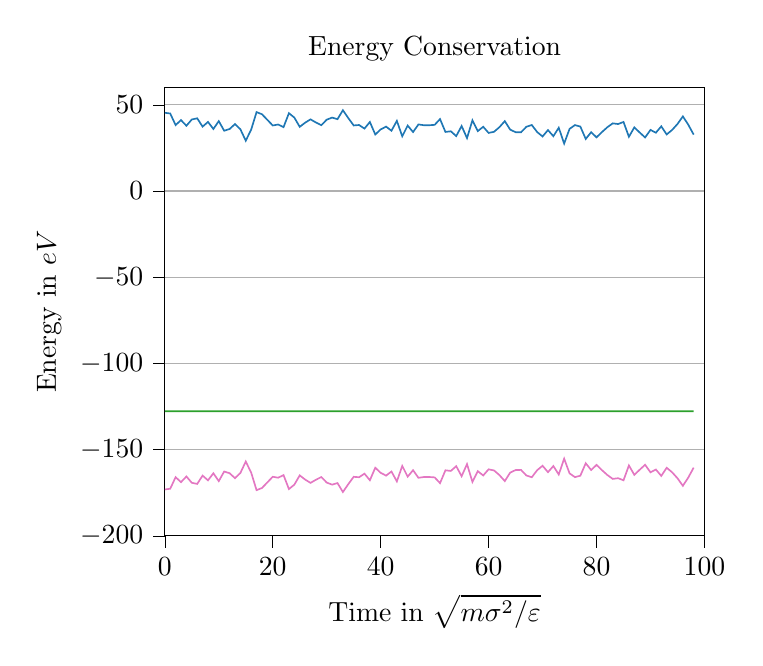
\begin{tikzpicture}

\definecolor{darkgray176}{RGB}{176,176,176}
\definecolor{forestgreen4416044}{RGB}{44,160,44}
\definecolor{orchid227119194}{RGB}{227,119,194}
\definecolor{steelblue31119180}{RGB}{31,119,180}

\begin{axis}[
tick align=outside,
tick pos=left,
title={Energy Conservation},
x grid style={darkgray176},
xlabel={Time in \(\displaystyle \sqrt{m \sigma^2 / \varepsilon}\)},
xmin=0, xmax=100,
xtick style={color=black},
y grid style={darkgray176},
ylabel={Energy in \(\displaystyle eV\)},
ymajorgrids,
ymin=-200, ymax=60,
ytick style={color=black}
]
\addplot [semithick, orchid227119194]
table {%
0 -173.092
1 -172.656
2 -165.957
3 -168.822
4 -165.549
5 -169.193
6 -169.878
7 -165.037
8 -167.782
9 -163.693
10 -168.245
11 -162.663
12 -163.652
13 -166.516
14 -163.528
15 -156.898
16 -163.273
17 -173.472
18 -172.239
19 -168.988
20 -165.71
21 -166.267
22 -164.752
23 -172.847
24 -170.297
25 -164.919
26 -167.327
27 -169.266
28 -167.447
29 -165.864
30 -169.079
31 -170.287
32 -169.373
33 -174.562
34 -170.007
35 -165.729
36 -165.989
37 -163.919
38 -167.74
39 -160.47
40 -163.433
41 -165.046
42 -162.676
43 -168.408
44 -159.409
45 -165.674
46 -161.896
47 -166.317
48 -165.868
49 -165.854
50 -166.077
51 -169.418
52 -161.963
53 -162.345
54 -159.573
55 -165.406
56 -158.383
57 -168.671
58 -162.472
59 -164.966
60 -161.399
61 -162.044
62 -164.719
63 -168.234
64 -163.292
65 -161.83
66 -161.725
67 -164.968
68 -166.005
69 -161.901
70 -159.327
71 -163.056
72 -159.499
73 -164.409
74 -155.217
75 -163.735
76 -165.936
77 -165.092
78 -157.894
79 -161.802
80 -158.829
81 -161.875
82 -164.684
83 -166.948
84 -166.553
85 -167.756
86 -159.154
87 -164.585
88 -161.626
89 -158.763
90 -163.143
91 -161.52
92 -165.233
93 -160.504
94 -163.106
95 -166.564
96 -170.975
97 -166.178
98 -160.41
};
\addplot [semithick, steelblue31119180]
table {%
0 45.3916
1 44.9558
2 38.2572
3 41.1212
4 37.8496
5 41.4928
6 42.1774
7 37.3373
8 40.082
9 35.9933
10 40.5449
11 34.9635
12 35.9521
13 38.8162
14 35.8279
15 29.1986
16 35.5732
17 45.7721
18 44.539
19 41.2875
20 38.0101
21 38.5671
22 37.0521
23 45.1469
24 42.5966
25 37.2193
26 39.6269
27 41.5654
28 39.7468
29 38.164
30 41.3786
31 42.5868
32 41.6724
33 46.8614
34 42.3065
35 38.0285
36 38.2893
37 36.2189
38 40.0397
39 32.7703
40 35.7326
41 37.346
42 34.9757
43 40.7082
44 31.7091
45 37.9738
46 34.1954
47 38.6169
48 38.1682
49 38.1541
50 38.3762
51 41.7178
52 34.2632
53 34.6447
54 31.8729
55 37.7062
56 30.6833
57 40.9706
58 34.7724
59 37.2656
60 33.699
61 34.3436
62 37.019
63 40.5337
64 35.5917
65 34.1304
66 34.0253
67 37.2679
68 38.3045
69 34.2013
70 31.6264
71 35.356
72 31.7987
73 36.7092
74 27.5173
75 36.0352
76 38.2364
77 37.3924
78 30.1941
79 34.102
80 31.1285
81 34.1754
82 36.9841
83 39.2482
84 38.8533
85 40.0564
86 31.4543
87 36.8848
88 33.9264
89 31.0628
90 35.4431
91 33.8203
92 37.5331
93 32.8039
94 35.4063
95 38.8634
96 43.2743
97 38.4771
98 32.7099
};
\addplot [semithick, forestgreen4416044]
table {%
0 -127.7
1 -127.701
2 -127.7
3 -127.7
4 -127.7
5 -127.7
6 -127.7
7 -127.7
8 -127.7
9 -127.7
10 -127.7
11 -127.7
12 -127.7
13 -127.7
14 -127.7
15 -127.7
16 -127.7
17 -127.7
18 -127.7
19 -127.7
20 -127.7
21 -127.7
22 -127.7
23 -127.7
24 -127.7
25 -127.7
26 -127.7
27 -127.7
28 -127.7
29 -127.7
30 -127.7
31 -127.7
32 -127.7
33 -127.7
34 -127.7
35 -127.7
36 -127.7
37 -127.7
38 -127.7
39 -127.7
40 -127.7
41 -127.7
42 -127.7
43 -127.7
44 -127.7
45 -127.7
46 -127.7
47 -127.7
48 -127.7
49 -127.7
50 -127.701
51 -127.701
52 -127.7
53 -127.7
54 -127.7
55 -127.7
56 -127.7
57 -127.7
58 -127.7
59 -127.7
60 -127.7
61 -127.7
62 -127.7
63 -127.7
64 -127.7
65 -127.7
66 -127.7
67 -127.7
68 -127.7
69 -127.7
70 -127.7
71 -127.7
72 -127.7
73 -127.7
74 -127.7
75 -127.7
76 -127.7
77 -127.7
78 -127.7
79 -127.7
80 -127.7
81 -127.7
82 -127.7
83 -127.7
84 -127.7
85 -127.7
86 -127.7
87 -127.7
88 -127.7
89 -127.7
90 -127.7
91 -127.7
92 -127.7
93 -127.7
94 -127.7
95 -127.7
96 -127.7
97 -127.701
98 -127.7
};
\draw (axis cs:103,-160.41) node[
  scale=0.5,
  anchor=west,
  text=orchid227119194,
  rotate=0.0
]{$E_\mathrm{pot}$};
\draw (axis cs:103,32.7098999999999) node[
  scale=0.5,
  anchor=west,
  text=steelblue31119180,
  rotate=0.0
]{$E_\mathrm{kin}$};
\draw (axis cs:103,-127.7) node[
  scale=0.5,
  anchor=west,
  text=forestgreen4416044,
  rotate=0.0
]{$E_\mathrm{total}$};
\end{axis}

\end{tikzpicture}
